On dispose d'une liste de joueurs d'un tournoi de tennis sous phase de poules (exemple : \textit{Master cup}), et on veut créer une liste de matches, de telle sorte que chaque joueur joue contre tous les autres joueurs une seule fois (pas de phase retour).

\begin{center}
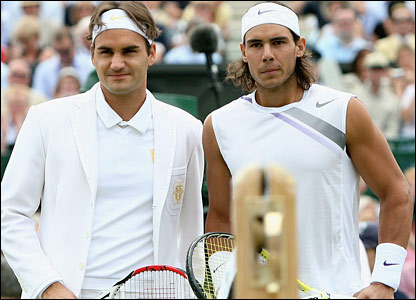
\includegraphics[width=.5\textwidth]{nadal-federer.jpg}
\end{center}

On peut découper ce problème en sous-problèmes plus simples imbriqués les uns dans les autres :
\begin{itemize}
\item On peut ainsi remarquer que si on a une liste de 4 joueurs, on peut résoudre le problème en connaissant une liste de matches pour les 3 premiers joueurs seulement : on prend cette liste, et on y ajoute un match entre le quatrième joueur et chacun des trois autres.


\item On peut programmer ce problème avec une fonction récursive dans Python :

\begin{itemize}
\item Soit la liste des joueurs notée "\textit{joueurs}"
\item Il faut commencer par initialiser le problème :

\textbf{s'il n'y a qu'un seul joueur, on n'organise aucun match.}


\item Il faut donner une relation de récurrence (récurcivité) :
on enlève le dernier joueur de la liste, et on demande les matches sans ce dernier.
\end{itemize}


\item Ici il faut penser à ajouter les sous-problèmes en ajoutant un match entre lui et tous les autres joueurs et donc à construire une liste de matches.
\item On remet le dernier joueur dans la liste des joueurs, et on renvoie la liste des matches.
\end{itemize}



On pourra utiliser la fonction .pop(), qui placée après une liste retire son dernier terme :

\begin{lstlisting}
joueurs=list(range(1,5))
joueurs.pop()
4
joueurs
[1, 2, 3]
\end{lstlisting}
De la même manière, on pourra utiliser la fonction \textbf{.append()}, qui placée après une liste ajoute un terme :

\begin{lstlisting}
joueurs=list(range(1,5))
joueurs.append(5)
joueurs
[1, 2, 3, 4, 5]
\end{lstlisting}

\question{} Écrire une fonction \texttt{matches(joueurs:list)->list} prenant en argument une liste de numéros de joueurs et renvoyant une listes de matchs sous la forme de couple de joueurs.



